% DONE, final typo check remaining

% --------------------------------------------------------------------
% Cheatsheet:
% \verb!lazy val!   -- esim. lyhyisiin koodinpätkiin
% \begin{verbatim}  -- esim. pitkiin koodinpätkiin
% `` tekstiä ''     -- lainausmerkit
% \textbf{huom!}    -- boldaus
% \begin{quotation}
% \noindent \it     -- quoten lisäys
% \ldots            -- kolme pistettä
% footnote{juh}     -- alaviite
% \citet, \citep
% \citet[s.234]{}   -- viitteet, http://merkel.zoneo.net/Latex/natbib.php
% \begin{sloppypar} -- ahdas teksti
% \clearpage        -- onkkelmien korjaamiseen lukujen kanssa
% --                -- yhdysviiva
% \enumerate
% \itemize          -- listat
% \begin[htb]{figure}
% \begin[htb]{table} - Kuva ja taulukko, (h)ere, (t)op, (b)ottom
% \begin{equation}  -- kaava
% \label{eq:kaava1} -- laabeli
%!TEX root = main.tex

\section{Laiskan evaluoinnin kehitys \label{historia}}

Normaalijärjestyksessä evaluoinnin periaate syntyi 1970-luvulla. Sarja julkaisuja loi pohjaa ajatukselle ``laiskoista'' funktionaalisista kielistä työkaluna käytännönläheiseen ohjelmistokehitykseen. Ajatus esiteltiin ensimmäisenä matemaattisesti lambdakalkyylin, funktionaalisen ohjelmoinnin kannalta keskeisen matemaattisen teorian, näkökulmasta \citep{wadsworth1971semantics}. Viisi vuotta myöhemmin julkaistiin toisistaan riippumatta kolme artikkelia \citep{henderson1976lazy,friedman1976cuns,saslmanualturner}, joissa esiteltiin normaalijärjestyksessä laiskaa evaluointia  funktionaalisen ohjelmoinnin perspektiivistä.

\subsection{Haskellin ja puhtaan funktionaalisen ohjelmoinnin kehitys}

\citet{hudak2007history} kuvaa, kuinka 1980-luvun puolivälissä laiskaa evaluointia (joka tuolloin käytännössä tarkoitti käytännössä normaalijärjestyksessä evaluointia) hyödyntävien ohjelmointikielien määrä kasvoi nopeasti. Useimmat kielistä soveltuivat vain kapeaan määrään käyttökohteita, ja niiden käyttäjämäärä oli pieni. Kuitenkin artikkelin kirjoittajat olivat tällöin sitä mieltä, että kielet muistuttivat ominaisuuksiltaan hyvin paljon toisiaan. Alkoi kehittyä ajatus siitä, että olisi hyvä luoda yksi, yleinen kieli, joka korvaisi kerralla monia aikaisempia kieliä.

Tämä johti Haskell-ohjelmointikielen kehityksen aloittamiseen. Siitä vastasi Haskell-komitea, jossa vaikutti monia aikaisempien laiskaa evaluointia hyödyntäneiden kielien suunnittelijoita. Komitea onnistui keräämään yhteen aikaisemmin erillään samaa aihepiiriä tutkineita, mikä kiihdytti laiskan evaluoinnin piirissä olevien evaluointisemantiikkojen tieteellistä kehitystä. Alkuvaiheen kehitystyö oli onnistunutta, ja Haskellista kehittyi etenkin tietojenkäsittelytieteen akateemisen tutkimuksen parissa suosittu kieli.

Haskell ei määritelmällisesti ole normaalijärjestyksessä evaluoitu ohjelmointikieli, vaan jo Haskell 1.1 -raportissa \citep{yale1991report} se määriteltiin ainoastaan ei-tiukkaa semantiikan määritelmän täyttäväksi kieleksi. Käytännössäkään kielessä funktioiden parametreja ei aina evaluoida vasta kun ohjelmakoodi niitä tarvitsee, vaan Haskellin kääntäjät tekevät useita nopeusoptimointeja suorittamalla tiettyjä osia koodista tiukan semantiikan säännöllä.

Useimmat kielen rakenteet noudattavat kuitenkin oletusarvoisesti call-by-need –evaluointisemantiikan sääntöjä, eli funktioiden argumenttilausekkeet evaluoidaan vasta sitten niitä kuin tarvitaan, ja evaluoidut arvot muistioidaan. Listauksessa \ref{code-callbyneed-haskell} on esimerkki siitä, miten call-by-need -semantiikka näkyy käytännössä Haskellissa.

\begin{listing}[H]
  \caption{Esimerkki call-by-need -semantiikasta Haskellissa}
  \label{code-callbyneed-haskell}
  \bigskip
  \begin{minted}[linenos=false, xleftmargin=0pt]{haskell}
> -- Tämä esimerkki ajetaan Haskellin komentoriviversiossa eli REPLissä
> -- Luodaan kokonaisluvuista koostuva lista, jolla on kaksi alkiota
> let list = [5 * 5, 5 + 5] :: [Integer]
> -- Tulostetaan listan arvo ja huomataan, että alkioita ei vielä ole evaluoitu
> -- Merkki `_` kertoo, että arvoa ei ole evaluoitu
> :sprint list
[_,_]
> -- Tulostetaan listan ensimmäinen arvo
> -- (erillistä `print` -kutsua ei REPlissä tarvita)
> head list
25
> -- Nyt ensimmäinen arvo on muistioitu, eli se voidaan palauttaa suoraan muistista,
> -- ja vain toinen arvo on evaluoimatta
> :sprint list
[25,_]
> -- Tulostetaan listan kaikki arvot
> -- Ensimmäinen arvo palautetaan muistista ja toinen evaluoidaan
> list
[25,10]
> :sprint list
[25,10]
\end{minted}
\end{listing}

Call-by-need -evaluointisemantiikka aiheuttaa sen, että ohjelmointikielen lausekkeiden evaluointi etenee erilaisessa järjestyksessä kuin applikatiivisesti evaluoiduissa kielissä. Call-by-need -semantiikan kielissä järjestys, jossa ohjelmakoodin rivit on kirjoitettu, ei vielä kerro suoritusjärjestystä, vaan suoritusjärjestys määräytyy dynaamisesti ohjelman suorituksen aikana.

Yksi merkittävä käytännön seuraus tästä on, että IO-operaatioita, eli esimerkiksi näytölle tulostamista tai käyttäjän syötteen odottamista, ei pystytä suorittamaan halutussa järjestyksessä pelkkien tavallisten funktiokutsujen avulla. Siksi Haskelliin on kehitetty uniikkeja ohjelmointikielen rakenteita, kuten \textit{monadit}, joilla IO-operaatioita ja niiden järjestystä pystyy kontrolloimaan erillään muusta ohjelmakoodista.

Toinen seuraus call-by-need -evaluointisemantiikasta on se, että funktion parametrien arvoja ei ole mahdollista jälkikäteen muuttaa, koska suoritusjärjestys määräytyy dynaamisesti ja parametrin arvon muutokset voisivat tapahtua arvaamattomassa järjestyksessä. Siten funktionaalisen ohjelmoinnin ajatusmaailma etenkin referentiaalisen läpinäkyvyyden osalta sopii hyvin call-by-need -semantiikan kanssa yhteen. Haskell tukee puhtaasti funktionaalista ohjelmointityyliä kattavasti, sillä Haskellin funktioissa ei ole sivuvaikutuksia muutoin kuin monadien tarjoaman rajapinnan kautta.

\subsection{Haskellissa kääntäjän suunnittelussa tehdyt tekniset valinnat}

Laiskan evaluoinnin kokonaisvaltaisessa tarkastelussa on olennaista myös käydä läpi sitä, miten se on ohjelmointikielen kääntäjissä toteutettu, ja millaisia seurauksia sillä on ohjelman suorituksen aikaiseen käyttäytymiseen. Haskell-ohjelmointikielen ylivoimaisesti suosituin kääntäjä on ollut Glasgow Haskell Compiler (lyhyemmin GHC), joka on ollut 1990-luvun alusta lähtien ollut olennainen osa ohjelmointikielen kehityskaarta.

Kuten edellä mainittiin, Haskell-yhteisö tarkoittaa laiskalla evaluoinnilla yleensä call-by-need -evaluointisemantiikkaa. Call-by-need -semantiikka on GHC:ssä toteutettu siten, että ohjelman suorituksen aikana kielen lausekkeista muodostetaan dynaamisesti verkkoa, jossa yksittäistä evaluoimatonta lauseketta kutsutaan \textit{tyngiksi} (eng. \textit{thunk}) \citep{hudak2007history}. Näitä tynkiä evaluoidaan sitä mukaan, kun jokin ohjelman IO-operaatio tarvitsee niiden arvoja. Kuvassa \ref{figure:thunk} näytetään, miten erään yksinkertaisen tietorakenteen evaluointi etenee.
\begin{figure}[h]
  \centering
    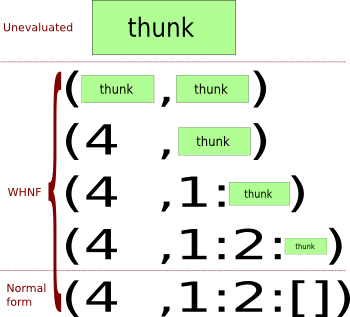
\includegraphics[width=0.3\textwidth]{figure-thunk-layers}
  \caption{\footnotesize\textbf{Lausekkeen (4, [1, 2]) evaluointi Haskellissa.} Ensiksi lauseke on kokonaan evaluoimatta. Se evaluoidaan asteittain, kunnes tynkiä ei ole jäljellä. Kokonaan evaluoidusta lausekkeesta sanotaan, että se on \textit{normaalimuodossa}. Lauseketta, joka on ainakin osittain evaluoitu, kutsutaan \textit{heikoksi päänormaalimuodoksi} (eng. \textit{Weak Head Normal Form}). Kuvan lähde on \citet{wikicommonsthunk}.}
  \label{figure:thunk}
\end{figure}

Tämä toteutus eroaa monista applikatiivisesti evaluoiduista kielistä etenkin siinä, että tynkien muodostava verkko voi itsessään viedä ohjelman suoritusaikana huomattavasti muistia. Lisäksi se, että jokin IO-operaatio tarvitsee jonkin tyngän arvoa, voi aiheuttaa hetkellisen hidastumisen ohjelman suoritukseen, jos sisäkkäisiä evaluoimattomia tynkiä on kertynyt paljon. Kumpaakaan näistä ilmiöistä ei esiinny applikatiivisen evaluoinnin kielissä, sillä niissä lausekkeet suoritetaan siinä järjestyksessä missä ne on ohjelmakoodiin kirjoitettu, ja tynkiä ei tarvita.

\subsection{Leviäminen muihin ohjelmointikieliin}

Haskell on nykypäivänä suosituista ohjelmointikielistä ainoita, joissa applikatiivinen evaluointisemantiikka on rakennettu perustavanlaatuiseksi osaksi kielen toteutusta. Kuitenkin monet Haskellissa esitellyt ideat ovat levinneet myös muihin kieliin. Käsittelen näitä ideoita ja niiden sovelluksia eri ohjelmointikielissä seuraavassa luvussa.
